% Options for packages loaded elsewhere
\PassOptionsToPackage{unicode}{hyperref}
\PassOptionsToPackage{hyphens}{url}
%
\documentclass[
]{report}
\usepackage{amsmath,amssymb}
\usepackage{iftex}
\ifPDFTeX
  \usepackage[T1]{fontenc}
  \usepackage[utf8]{inputenc}
  \usepackage{textcomp} % provide euro and other symbols
\else % if luatex or xetex
  \usepackage{unicode-math} % this also loads fontspec
  \defaultfontfeatures{Scale=MatchLowercase}
  \defaultfontfeatures[\rmfamily]{Ligatures=TeX,Scale=1}
\fi
\usepackage{lmodern}
\ifPDFTeX\else
  % xetex/luatex font selection
\fi
% Use upquote if available, for straight quotes in verbatim environments
\IfFileExists{upquote.sty}{\usepackage{upquote}}{}
\IfFileExists{microtype.sty}{% use microtype if available
  \usepackage[]{microtype}
  \UseMicrotypeSet[protrusion]{basicmath} % disable protrusion for tt fonts
}{}
\makeatletter
\@ifundefined{KOMAClassName}{% if non-KOMA class
  \IfFileExists{parskip.sty}{%
    \usepackage{parskip}
  }{% else
    \setlength{\parindent}{0pt}
    \setlength{\parskip}{6pt plus 2pt minus 1pt}}
}{% if KOMA class
  \KOMAoptions{parskip=half}}
\makeatother
\usepackage{xcolor}
\usepackage[margin=3.5cm]{geometry}
\usepackage{graphicx}
\makeatletter
\def\maxwidth{\ifdim\Gin@nat@width>\linewidth\linewidth\else\Gin@nat@width\fi}
\def\maxheight{\ifdim\Gin@nat@height>\textheight\textheight\else\Gin@nat@height\fi}
\makeatother
% Scale images if necessary, so that they will not overflow the page
% margins by default, and it is still possible to overwrite the defaults
% using explicit options in \includegraphics[width, height, ...]{}
\setkeys{Gin}{width=\maxwidth,height=\maxheight,keepaspectratio}
% Set default figure placement to htbp
\makeatletter
\def\fps@figure{htbp}
\makeatother
\ifLuaTeX
  \usepackage{luacolor}
  \usepackage[soul]{lua-ul}
\else
  \usepackage{soul}
\fi
\setlength{\emergencystretch}{3em} % prevent overfull lines
\providecommand{\tightlist}{%
  \setlength{\itemsep}{0pt}\setlength{\parskip}{0pt}}
\setcounter{secnumdepth}{-\maxdimen} % remove section numbering
\usepackage{eso-pic,graphicx,transparent}
\usepackage{fancyhdr}
\usepackage{lastpage}
\pagestyle{fancy}
\fancyhead[RO,RE]{\thepage\ of \pageref{LastPage}}
\fancyfoot{}
\vspace{-0.5em}

\includegraphics[width=2in,height=2in]{MoPIED_Logo.png}\LARGE\\}
\usepackage{booktabs}
\usepackage{longtable}
\usepackage{array}
\usepackage{multirow}
\usepackage{wrapfig}
\usepackage{float}
\usepackage{colortbl}
\usepackage{pdflscape}
\usepackage{tabu}
\usepackage{threeparttable}
\usepackage{threeparttablex}
\usepackage[normalem]{ulem}
\usepackage{makecell}
\usepackage{xcolor}
\ifLuaTeX
  \usepackage{selnolig}  % disable illegal ligatures
\fi
\usepackage{bookmark}
\IfFileExists{xurl.sty}{\usepackage{xurl}}{} % add URL line breaks if available
\urlstyle{same}
\hypersetup{
  pdftitle={Methodology for Prioritizing IDP Solutions in Somalia},
  pdfauthor={DTM - Data for Solution},
  hidelinks,
  pdfcreator={LaTeX via pandoc}}

\title{Methodology for Prioritizing IDP Solutions in Somalia}
\usepackage{etoolbox}
\makeatletter
\providecommand{\subtitle}[1]{% add subtitle to \maketitle
  \apptocmd{\@title}{\par {\large #1 \par}}{}{}
}
\makeatother
\subtitle{A Policy Brief on Data-Driven Decision Making for Durable
Solutions}
\author{DTM - Data for Solution}
\date{2024-10-29}

\begin{document}
\maketitle

{
\setcounter{tocdepth}{3}
\tableofcontents
}
\AddToShipoutPictureFG{
\AtPageCenter{% or \AtTextCenter
\makebox[0pt]{\rotatebox[origin=c]{45}{%
\scalebox{10}{\texttransparent{0.1}{DRAFT}}%
}}
}
}

\newpage

\chapter{Introduction}\label{introduction}

Somalia is currently grappling with a prolonged crisis, marked by
approximately 3.8 million internally displaced persons (IDPs). Many of
these individuals have migrated from rural areas to urban centers due to
a combination of environmental shocks, food insecurity, limited
livelihood opportunities, and ongoing armed conflict. In response to
this pressing issue, the Department of Poverty Reduction and Durable
Solutions within the Ministry of Planning, Investments, and Economic
Development (MoPIED) plays a pivotal role in managing and addressing
solutions for internal displacement throughout the country.

In 2024, the department organized a series of consultations on durable
solutions pathways across all federal member states and the Banadir
Regional Administration (BRA). The primary objective of these
consultations was to identify effective strategies to facilitate the
durable solutions pathways for one million IDPs, helping them transition
from their current displacement situations. This initiative aligns with
the National Durable Solutions Strategy, the National Development Plan,
and the United Nations Secretary-General's Action Agenda on Internal
Displacement. These frameworks emphasize three interconnected goals:
achieving durable solutions, ensuring protection and assistance, and
preventing future displacement.

The workshops held during these consultations were structured around
several fundamental elements designed to address the complex needs of
IDPs and facilitate durable solutions. The key elements forming the
foundation for durable solutions pathways include:

\begin{enumerate}
\def\labelenumi{\arabic{enumi}.}
\tightlist
\item
  \textbf{Solutions Pathway 1:} Government Leadership -- Strengthening
  governmental roles and responsibilities in implementing solutions.
\item
  \textbf{Solutions Pathway 2:} Access to Basic Services -- Ensuring
  that IDPs have access to essential services such as healthcare,
  education, and sanitation.
\item
  \textbf{Solutions Pathway 3:} Employment and Livelihood Opportunities
  -- Creating opportunities for sustainable livelihoods to enhance
  economic stability.
\item
  \textbf{Solutions Pathway 4:} Legal Documentation, Housing, Land, and
  Property (HLP) -- Addressing legal and housing issues to secure IDPs'
  rights to land and property.
\item
  \textbf{Solutions Pathway 5:} Addressing Climate Change and Building
  Resilience -- Focusing on strategies that mitigate the impacts of
  climate change and enhance community resilience.
\item
  \textbf{Solutions Pathway 6:} Data for Solutions: Generating Reliable
  Data -- Establishing reliable data collection methods to inform
  decision-making and policy formulation.
\end{enumerate}

This report outlines a comprehensive methodology aimed at identifying
priority locations for intervention specifically related to solutions
pathways 2 through 5.

\section{Research questions}\label{research-questions}

\begin{itemize}
\tightlist
\item
  Identify priority locations for government fundraising efforts aligned
  with solution pathways.
\item
  Identify target demographic groups for each solution pathway
\end{itemize}

\section{Limitation}\label{limitation}

\begin{enumerate}
\def\labelenumi{\arabic{enumi}.}
\item
  In Somalia, there is a notable trend of internally displaced persons
  (IDPs) increasingly relocating to larger cities in search of better
  access to essential services and facilities. This influx places a
  significant burden on urban areas, which are often ill-equipped to
  support the high number of IDPs. As a result, the strain on resources
  in these cities can lead to overcrowding, increased competition for
  jobs, and heightened tension between IDPs and local residents.
  Research indicates that if essential services were made available in
  relatively smaller cities, a significant number of IDPs would be more
  likely to settle there instead of migrating to larger urban centers.
  This shift could alleviate some of the pressure on big cities while
  simultaneously fostering more balanced regional development. By
  investing in infrastructure and service provision in smaller towns,
  policymakers could create environments that attract IDPs, thus
  promoting their well-being and integration into local communities.
  However, the methods proposed in this report do not take this crucial
  aspect into account when determining intervention priorities.
\item
  This methodology operates under the assumption that the data for all
  indicators related to each pathway is sourced from a single, unified
  data set
\end{enumerate}

\chapter{Methodology}\label{methodology}

\section{Overview}\label{overview}

The methodology utilizes a comprehensive multi-tiered scoring system
designed to assess the current situation across various pathways. Each
pathway encompasses several sub-criteria, which are composed of
distinct, measurable indicators. This approach allows for a nuanced
evaluation, as it breaks down each pathway into specific elements that
can be quantified and analyzed.This structured methodology aims to
provide a clear, detailed understanding of the current landscape,
supporting informed decision-making and strategic planning.

\section{Data Processing Steps}\label{data-processing-steps}

Initially, each pathway will have multiple sub-indicators selected, with
various indicators chosen under each sub-criterion. All indicators will
then be converted to binary values, with ``Pass'' assigned a value of 1
and ``Fail'' a value of 0. Responses such as ``Don't know'' or ``Prefer
not to say'' will be classified as ``NA.'' Generally, ``NA'' responses
will remain as such, though specific questions may require recoding
these as ``Pass'' or ``Fail'' based on predetermined conditions. After
recoding, sub-criteria scores will be calculated by applying equal
weights and standardizing them on a 0--1 scale. Scores below 0.50 will
be recorded as 0, while scores equal to or above 0.50 will be recorded
as 1. This same methodology will be used to compute final pathway scores
based on the sub-criteria.

\section{Case Study: HLP and Documentation (solutions pathway
4)}\label{case-study-hlp-and-documentation-solutions-pathway-4}

\subsection{Step 1: Indentifying the list of
indicators}\label{step-1-indentifying-the-list-of-indicators}

Let's take an example of HLP and documentation (solution pathway 4).
Within this pathway, we have identified the following two sub-criteria
and five indicators.

\begin{itemize}
\item
  {[}Sub indicator{]} \ul{4.1 HLP}
\item
  4.1.1 \% of households with a written agreement or land title deed for
  the land they occupy.
\item
  4.1.2 \% of households reporting that no one attempted to evict them
  from their property in the past three months.
\item
  4.1.3 \% of households facing negligible or no risk of eviction from
  their current property or land.
\item
  4.1.4 \% of households that have never or rarely been involved in
  disputes or conflicts related to access to the land they occupy in the
  past three months.
\item
  {[}Sub indicator{]} \ul{4.2 Documentation}
\item
  4.2.1 \% of households with either a birth certificate, ID, passport,
  or marriage certificate.
\end{itemize}

In the next sections we will create a comprehensive matrix step by step
for HLP and Documentation pathways using \textbf{dummay data}

\subsection{Step 2: Collect household-level data for all
indicators}\label{step-2-collect-household-level-data-for-all-indicators}

The next step after identifying the indicators is to collect
household-level data for each indicator by city. Potential data sources
include:

\begin{enumerate}
\def\labelenumi{\arabic{enumi}.}
\tightlist
\item
  Durable Solution Progress (DSP) Survey
\item
  Service Analysis and Mapping
\item
  Area-Based Assessments
\item
  MSNA
\end{enumerate}

\emph{However, for this purpose, the DSP and Service Analysis and
Mapping may be more suitable, as these two surveys are specifically
designed to gather information at the neighborhood level.}

Let's assume we have the following dataset that includes all indicators
for solution pathway 4: HLP and legal documentation.

\begin{longtable}[t]{lllll}
\caption{\label{tab:hh_data}Sample HH data for seleted indicators}\\
\toprule
HH\_id & Ind-4.1.1 & Ind-4.1.2 & Ind-4.1.3 & Ind-4.1.4\\
\midrule
1 & Verbal agreement & Facing eviction thread & High risk & Often\\
2 & Written agreement & No eviction thread & Low risk & Never\\
3 & No agreement & Facing eviction thread & High risk & Sometimes\\
4 & Dont know & No eviction thread & Negligible & Rarely\\
5 & Verbal agreement & Facing eviction thread & No risk & Never\\
\bottomrule
\end{longtable}

Now we will recode the data according to the definitions established in
Step 1. The rules will be as follows:

\begin{enumerate}
\def\labelenumi{\arabic{enumi}.}
\tightlist
\item
  Ind-4.1.1:
\end{enumerate}

\begin{itemize}
\tightlist
\item
  Pass (1): Written agreement and land title deed
\item
  Fail (0): No agreement, verbal agreement
\item
  NA: Don't know/Prefer not to say
\end{itemize}

\begin{enumerate}
\def\labelenumi{\arabic{enumi}.}
\setcounter{enumi}{1}
\tightlist
\item
  Ind-4.1.2:
\end{enumerate}

\begin{itemize}
\tightlist
\item
  Pass (1): No eviction threat
\item
  Fail (0): Facing eviction threat
\item
  NA: Don't know/Prefer not to say
\end{itemize}

\begin{enumerate}
\def\labelenumi{\arabic{enumi}.}
\setcounter{enumi}{2}
\tightlist
\item
  Ind-4.1.3:
\end{enumerate}

\begin{itemize}
\tightlist
\item
  Pass (1): No risk or negligible
\item
  Fail (0): Low or high risk
\item
  NA: Don't know/Prefer not to say
\end{itemize}

\begin{enumerate}
\def\labelenumi{\arabic{enumi}.}
\setcounter{enumi}{3}
\tightlist
\item
  Ind-4.1.4:
\end{enumerate}

\begin{itemize}
\tightlist
\item
  Pass (1): Never or rarely
\item
  Fail (0): Often or sometimes
\item
  NA: Don't know/Prefer not to say
\end{itemize}

\begin{longtable}[t]{ccccc}
\caption{\label{tab:indicator_recoding}Indicator Recoding to Binary Value}\\
\toprule
HH\_id & Ind-4.1.1 & Ind-4.1.2 & Ind-4.1.3 & Ind-4.1.4\\
\midrule
1 & 0 & 0 & 0 & 0\\
2 & 1 & 1 & 0 & 1\\
3 & 0 & 0 & 0 & 0\\
4 & NA & 1 & 1 & 1\\
5 & 0 & 0 & 1 & 1\\
\bottomrule
\end{longtable}

\subsection{Step 3: Create composite indicator at sub-criteria
level}\label{step-3-create-composite-indicator-at-sub-criteria-level}

In this example, we will now create a composite score for the
sub-criteria using the following equation:

\begin{equation}
`Sub Criteria` = (`Sum of all non-NA indicators`)/(`Number of non-NA indicators`)
\end{equation}

\newpage

\begin{longtable}[t]{ccccc>{}c}
\caption{\label{tab:compisite}Sub-Criteria Calculation for HLP and Documentation Pathway}\\
\toprule
HH\_id & Ind-4.1.1 & Ind-4.1.2 & Ind-4.1.3 & Ind-4.1.4 & Sub-ind-4.1\\
\midrule
1 & 0 & 0 & 0 & 0 & \cellcolor{cyan}{\textcolor{black}{\textbf{0.00}}}\\
2 & 1 & 1 & 0 & 1 & \cellcolor{cyan}{\textcolor{black}{\textbf{0.75}}}\\
3 & 0 & 0 & 0 & 0 & \cellcolor{cyan}{\textcolor{black}{\textbf{0.00}}}\\
4 & NA & 1 & 1 & 1 & \cellcolor{cyan}{\textcolor{black}{\textbf{1.00}}}\\
5 & 0 & 0 & 1 & 1 & \cellcolor{cyan}{\textcolor{black}{\textbf{0.50}}}\\
\bottomrule
\end{longtable}

\subsection{Step 4: Applying recoding rule on composite
indicator}\label{step-4-applying-recoding-rule-on-composite-indicator}

Once the sub indicator is created, we will recode using the following
rule:

\begin{verbatim}
- If composite score >= 0.50 → Pass (1)
- If composite score < 0.50 → Fail (0)
\end{verbatim}

\begin{longtable}[t]{ccccc>{}c}
\caption{\label{tab:compisite_recode}Recoding Sub-Criteria for HLP and Documentation Pathway}\\
\toprule
HH\_id & Ind-4.1.1 & Ind-4.1.2 & Ind-4.1.3 & Ind-4.1.4 & Sub-ind-4.1\\
\midrule
1 & 0 & 0 & 0 & 0 & \cellcolor{cyan}{\textcolor{black}{\textbf{0}}}\\
2 & 1 & 1 & 0 & 1 & \cellcolor{cyan}{\textcolor{black}{\textbf{1}}}\\
3 & 0 & 0 & 0 & 0 & \cellcolor{cyan}{\textcolor{black}{\textbf{0}}}\\
4 & NA & 1 & 1 & 1 & \cellcolor{cyan}{\textcolor{black}{\textbf{1}}}\\
5 & 0 & 0 & 1 & 1 & \cellcolor{cyan}{\textcolor{black}{\textbf{1}}}\\
\bottomrule
\end{longtable}

\subsection{Step 5: Applying same calculations for all sub criteria for
each
pathway}\label{step-5-applying-same-calculations-for-all-sub-criteria-for-each-pathway}

Using the same calculation method, we will calculate the scores for all
sub-criteria. In this specific example, we will calculate the remaining
sub-criteria \texttt{(Sub-Ind-4.2)} for HLP and documents.

\begin{longtable}[t]{ccccc>{}cc>{}c}
\caption{\label{tab:pathway_4_tbl}Sub-Criteria Score for HLP and Documentation Pathway}\\
\toprule
HH\_id & Ind-4.1.1 & Ind-4.1.2 & Ind-4.1.3 & Ind-4.1.4 & Sub-ind-4.1 & Ind-4.2.2 & Sub-ind-4.2\\
\midrule
1 & 0 & 0 & 0 & 0 & \cellcolor{cyan}{\textcolor{black}{\textbf{0}}} & 1 & \cellcolor{cyan}{\textcolor{black}{\textbf{1}}}\\
2 & 1 & 1 & 0 & 1 & \cellcolor{cyan}{\textcolor{black}{\textbf{1}}} & 0 & \cellcolor{cyan}{\textcolor{black}{\textbf{0}}}\\
3 & 0 & 0 & 0 & 0 & \cellcolor{cyan}{\textcolor{black}{\textbf{0}}} & 0 & \cellcolor{cyan}{\textcolor{black}{\textbf{0}}}\\
4 & NA & 1 & 1 & 1 & \cellcolor{cyan}{\textcolor{black}{\textbf{1}}} & 0 & \cellcolor{cyan}{\textcolor{black}{\textbf{0}}}\\
5 & 0 & 0 & 1 & 1 & \cellcolor{cyan}{\textcolor{black}{\textbf{1}}} & 1 & \cellcolor{cyan}{\textcolor{black}{\textbf{1}}}\\
\bottomrule
\end{longtable}

\subsection{Step 6: Calculating total
score}\label{step-6-calculating-total-score}

Once we have score for all sub criteria, we will calculate the pathway
score by applying simple sum.

\begingroup\fontsize{8}{10}\selectfont

\begin{longtable}[t]{ccccc>{}cc>{}c>{}c}
\caption{\label{tab:pathway_4_tbl_total}Total Score for HLP and Documentation Pathway}\\
\toprule
HH\_id & Ind-4.1.1 & Ind-4.1.2 & Ind-4.1.3 & Ind-4.1.4 & Sub-ind-4.1 & Ind-4.2.2 & Sub-ind-4.2 & Total-Score\\
\midrule
1 & 0 & 0 & 0 & 0 & \cellcolor{cyan}{\textcolor{black}{\textbf{0}}} & 1 & \cellcolor{cyan}{\textcolor{black}{\textbf{1}}} & \cellcolor{teal}{\textcolor{black}{\textbf{1}}}\\
2 & 1 & 1 & 0 & 1 & \cellcolor{cyan}{\textcolor{black}{\textbf{1}}} & 0 & \cellcolor{cyan}{\textcolor{black}{\textbf{0}}} & \cellcolor{teal}{\textcolor{black}{\textbf{1}}}\\
3 & 0 & 0 & 0 & 0 & \cellcolor{cyan}{\textcolor{black}{\textbf{0}}} & 0 & \cellcolor{cyan}{\textcolor{black}{\textbf{0}}} & \cellcolor{teal}{\textcolor{black}{\textbf{0}}}\\
4 & NA & 1 & 1 & 1 & \cellcolor{cyan}{\textcolor{black}{\textbf{1}}} & 0 & \cellcolor{cyan}{\textcolor{black}{\textbf{0}}} & \cellcolor{teal}{\textcolor{black}{\textbf{1}}}\\
5 & 0 & 0 & 1 & 1 & \cellcolor{cyan}{\textcolor{black}{\textbf{1}}} & 1 & \cellcolor{cyan}{\textcolor{black}{\textbf{1}}} & \cellcolor{teal}{\textcolor{black}{\textbf{2}}}\\
\bottomrule
\end{longtable}
\endgroup{}

\subsection{Step 7: Creating City-Level Matrix for HLP and Documentation
Pathway}\label{step-7-creating-city-level-matrix-for-hlp-and-documentation-pathway}

Finally, we will develop a city-level matrix by calculating the
percentage of passes for each indicator and sub-indicator, as well as
the average total score for each city.

\begingroup\fontsize{8}{10}\selectfont

\begin{longtable}[t]{>{\centering\arraybackslash}p{.5in}>{}c>{}c>{}c>{}c>{}c>{}c>{}c>{\centering\arraybackslash}p{.4in}}
\caption{\label{tab:matrix}City-Level Matrix for HLP and Documentation Pathway}\\
\toprule
\multicolumn{1}{c}{ } & \multicolumn{5}{c}{\% passes Sub Indicator 1} & \multicolumn{2}{c}{\% passes Sub Indicator 2} & \multicolumn{1}{c}{ } \\
\cmidrule(l{3pt}r{3pt}){2-6} \cmidrule(l{3pt}r{3pt}){7-8}
City & Ind-4.1.1 & Ind-4.1.2 & Ind-4.1.3 & Ind-4.1.4 & Sub-ind-4.1 & Ind-4.2.2 & Sub-ind-4.2 & Total score (Mean)\\
\midrule
\textbf{Baardheere} & \textcolor[HTML]{440154}{\textbf{\textbf{40}}} & \textcolor[HTML]{355F8D}{\textbf{\textbf{50}}} & \textcolor[HTML]{FDE725}{\textbf{\textbf{88}}} & \textcolor[HTML]{440154}{\textbf{\textbf{35}}} & \textcolor[HTML]{482576}{\textbf{\textbf{70}}} & \textcolor[HTML]{3B528B}{\textbf{\textbf{55}}} & \textcolor[HTML]{3B528B}{\textbf{\textbf{55}}} & \textcolor[HTML]{306A8E}{\textbf{1.20}}\\
\textbf{Baydhaba} & \textcolor[HTML]{34618D}{\textbf{\textbf{56}}} & \textcolor[HTML]{25AB82}{\textbf{\textbf{67}}} & \textcolor[HTML]{50C46A}{\textbf{\textbf{80}}} & \textcolor[HTML]{B2DD2D}{\textbf{\textbf{66}}} & \textcolor[HTML]{50C46A}{\textbf{\textbf{88}}} & \textcolor[HTML]{50C46A}{\textbf{\textbf{76}}} & \textcolor[HTML]{50C46A}{\textbf{\textbf{76}}} & \textcolor[HTML]{1F9F88}{\textbf{1.40}}\\
\textbf{Berdaale} & \textcolor[HTML]{BDDF26}{\textbf{\textbf{87}}} & \textcolor[HTML]{440154}{\textbf{\textbf{34}}} & \textcolor[HTML]{20A486}{\textbf{\textbf{76}}} & \textcolor[HTML]{22A884}{\textbf{\textbf{56}}} & \textcolor[HTML]{440154}{\textbf{\textbf{67}}} & \textcolor[HTML]{3E4C8A}{\textbf{\textbf{54}}} & \textcolor[HTML]{3E4C8A}{\textbf{\textbf{54}}} & \textcolor[HTML]{440154}{\textbf{0.89}}\\
\textbf{Doolow} & \textcolor[HTML]{31B57B}{\textbf{\textbf{74}}} & \textcolor[HTML]{FDE725}{\textbf{\textbf{88}}} & \textcolor[HTML]{E7E419}{\textbf{\textbf{87}}} & \textcolor[HTML]{FDE725}{\textbf{\textbf{70}}} & \textcolor[HTML]{FDE725}{\textbf{\textbf{96}}} & \textcolor[HTML]{228B8D}{\textbf{\textbf{65}}} & \textcolor[HTML]{228B8D}{\textbf{\textbf{65}}} & \textcolor[HTML]{1F9F88}{\textbf{1.40}}\\
\textbf{Kismaayo} & \textcolor[HTML]{1F9E89}{\textbf{\textbf{69}}} & \textcolor[HTML]{470E61}{\textbf{\textbf{36}}} & \textcolor[HTML]{440154}{\textbf{\textbf{59}}} & \textcolor[HTML]{8BD646}{\textbf{\textbf{64}}} & \textcolor[HTML]{481B6D}{\textbf{\textbf{69}}} & \textcolor[HTML]{FDE725}{\textbf{\textbf{88}}} & \textcolor[HTML]{FDE725}{\textbf{\textbf{88}}} & \textcolor[HTML]{25AC82}{\textbf{1.45}}\\
\addlinespace
\textbf{MogDaynile} & \textcolor[HTML]{443B84}{\textbf{\textbf{49}}} & \textcolor[HTML]{77D153}{\textbf{\textbf{77}}} & \textcolor[HTML]{60CA60}{\textbf{\textbf{81}}} & \textcolor[HTML]{69CD5B}{\textbf{\textbf{62}}} & \textcolor[HTML]{31B57B}{\textbf{\textbf{86}}} & \textcolor[HTML]{50C46A}{\textbf{\textbf{76}}} & \textcolor[HTML]{50C46A}{\textbf{\textbf{76}}} & \textcolor[HTML]{20A486}{\textbf{1.42}}\\
\textbf{MogKahda} & \textcolor[HTML]{CAE11F}{\textbf{\textbf{88}}} & \textcolor[HTML]{297A8E}{\textbf{\textbf{56}}} & \textcolor[HTML]{75D054}{\textbf{\textbf{82}}} & \textcolor[HTML]{32B67A}{\textbf{\textbf{58}}} & \textcolor[HTML]{50C46A}{\textbf{\textbf{88}}} & \textcolor[HTML]{EFE51C}{\textbf{\textbf{87}}} & \textcolor[HTML]{EFE51C}{\textbf{\textbf{87}}} & \textcolor[HTML]{FDE725}{\textbf{1.80}}\\
\textbf{Xudur} & \textcolor[HTML]{FDE725}{\textbf{\textbf{92}}} & \textcolor[HTML]{21A685}{\textbf{\textbf{66}}} & \textcolor[HTML]{3C508B}{\textbf{\textbf{66}}} & \textcolor[HTML]{58C765}{\textbf{\textbf{61}}} & \textcolor[HTML]{443B84}{\textbf{\textbf{72}}} & \textcolor[HTML]{440154}{\textbf{\textbf{44}}} & \textcolor[HTML]{440154}{\textbf{\textbf{44}}} & \textcolor[HTML]{26828E}{\textbf{1.29}}\\
\bottomrule
\end{longtable}
\endgroup{}

\textbf{Interpretation:} The matrix above effectively addresses our
first research question. For instance, by examining the
\texttt{Total\ score\ (mean)} column, we can see that \texttt{Berdaale}
has the lowest score, indicating that it should be prioritized over
other cities for any HLP (Housing, Land, and Property) or
documentation-related projects. A closer look reveals that only
\texttt{34\%} of cases pass for indicator \texttt{4.1.2}, which assesses
the presence of solutions for eviction threats. This low pass rate
suggests that Berdaale urgently requires targeted HLP solutions to
address eviction risks, more so than other locations. Thus, the matrix
not only identifies priority areas but also highlights specific needs
within those areas to inform strategic project deployment.''

\subsection{Step 8: Normalizating the total
score}\label{step-8-normalizating-the-total-score}

Since solution paths have different numbers of subcriteria, their total
scores will naturally have different ranges. To make scores easily
comparable across all solution paths, we will normalize them to a 0-5
scale using the standard normalization equation:

\texttt{Total\ score} = ((\texttt{Total\ score(mean)} -
min)/(max-min))*5

\begingroup\fontsize{8}{10}\selectfont

\begin{longtable}[t]{cccccccc>{}c}
\caption{\label{tab:matrix2}City-Level Matrix for HLP and Documentation Pathway}\\
\toprule
City & Ind-4.1.1 & Ind-4.1.2 & Ind-4.1.3 & Ind-4.1.4 & Sub-ind-4.1 & Ind-4.2.2 & Sub-ind-4.2 & Total score\\
\midrule
Baardheere & 40 & 50 & 88 & 35 & 70 & 55 & 55 & \cellcolor{teal}{\textcolor{black}{\textbf{2}}}\\
Baydhaba & 56 & 67 & 80 & 66 & 88 & 76 & 76 & \cellcolor{teal}{\textcolor{black}{\textbf{3}}}\\
Berdaale & 87 & 34 & 76 & 56 & 67 & 54 & 54 & \cellcolor{teal}{\textcolor{black}{\textbf{0}}}\\
Doolow & 74 & 88 & 87 & 70 & 96 & 65 & 65 & \cellcolor{teal}{\textcolor{black}{\textbf{3}}}\\
Kismaayo & 69 & 36 & 59 & 64 & 69 & 88 & 88 & \cellcolor{teal}{\textcolor{black}{\textbf{3}}}\\
\addlinespace
MogDaynile & 49 & 77 & 81 & 62 & 86 & 76 & 76 & \cellcolor{teal}{\textcolor{black}{\textbf{3}}}\\
MogKahda & 88 & 56 & 82 & 58 & 88 & 87 & 87 & \cellcolor{teal}{\textcolor{black}{\textbf{5}}}\\
Xudur & 92 & 66 & 66 & 61 & 72 & 44 & 44 & \cellcolor{teal}{\textcolor{black}{\textbf{2}}}\\
\bottomrule
\end{longtable}
\endgroup{}

\subsection{Step 9: Defining the
priority}\label{step-9-defining-the-priority}

In the final stage, the cities will be classified into three priority
categories based on their scores:

\begin{figure}

{\centering 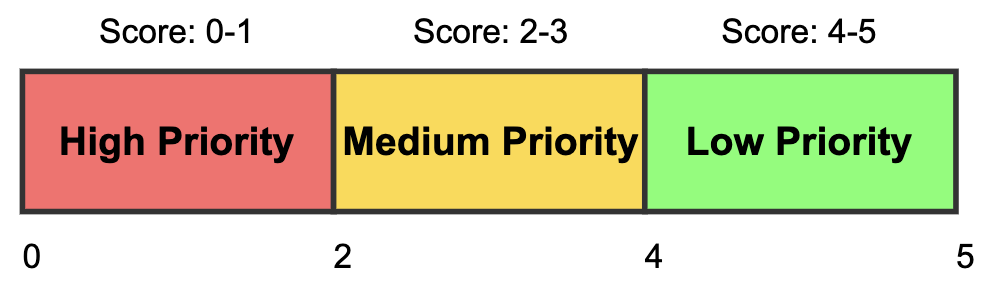
\includegraphics[width=3.33in]{priority} 

}

\caption{Priority category}\label{fig:svg-method1}
\end{figure}

Hence the we priority matrix will look like the following table:

\begingroup\fontsize{8}{10}\selectfont

\begin{longtable}[t]{ccccccccc}
\caption{\label{tab:matrix3}City-Level Priority Matrix for HLP and Documentation Pathway}\\
\toprule
City & Ind-4.1.1 & Ind-4.1.2 & Ind-4.1.3 & Ind-4.1.4 & Sub-ind-4.1 & Ind-4.2.2 & Sub-ind-4.2 & Priority level\\
\midrule
\endfirsthead
\caption[]{City-Level Priority Matrix for HLP and Documentation Pathway \textit{(continued)}}\\
\toprule
City & Ind-4.1.1 & Ind-4.1.2 & Ind-4.1.3 & Ind-4.1.4 & Sub-ind-4.1 & Ind-4.2.2 & Sub-ind-4.2 & Priority level\\
\midrule
\endhead

\endfoot
\bottomrule
\endlastfoot
\cellcolor[HTML]{ffd93d}{\textcolor{black}{\textbf{Baardheere}}} & \cellcolor[HTML]{ffd93d}{\textcolor{black}{\textbf{40}}} & \cellcolor[HTML]{ffd93d}{\textcolor{black}{\textbf{50}}} & \cellcolor[HTML]{ffd93d}{\textcolor{black}{\textbf{88}}} & \cellcolor[HTML]{ffd93d}{\textcolor{black}{\textbf{35}}} & \cellcolor[HTML]{ffd93d}{\textcolor{black}{\textbf{70}}} & \cellcolor[HTML]{ffd93d}{\textcolor{black}{\textbf{55}}} & \cellcolor[HTML]{ffd93d}{\textcolor{black}{\textbf{55}}} & \cellcolor[HTML]{ffd93d}{\textcolor{black}{\textbf{Medium}}}\\
\cellcolor[HTML]{ffd93d}{\textcolor{black}{\textbf{Baydhaba}}} & \cellcolor[HTML]{ffd93d}{\textcolor{black}{\textbf{56}}} & \cellcolor[HTML]{ffd93d}{\textcolor{black}{\textbf{67}}} & \cellcolor[HTML]{ffd93d}{\textcolor{black}{\textbf{80}}} & \cellcolor[HTML]{ffd93d}{\textcolor{black}{\textbf{66}}} & \cellcolor[HTML]{ffd93d}{\textcolor{black}{\textbf{88}}} & \cellcolor[HTML]{ffd93d}{\textcolor{black}{\textbf{76}}} & \cellcolor[HTML]{ffd93d}{\textcolor{black}{\textbf{76}}} & \cellcolor[HTML]{ffd93d}{\textcolor{black}{\textbf{Medium}}}\\
\cellcolor[HTML]{ff6b6b}{\textcolor{black}{\textbf{Berdaale}}} & \cellcolor[HTML]{ff6b6b}{\textcolor{black}{\textbf{87}}} & \cellcolor[HTML]{ff6b6b}{\textcolor{black}{\textbf{34}}} & \cellcolor[HTML]{ff6b6b}{\textcolor{black}{\textbf{76}}} & \cellcolor[HTML]{ff6b6b}{\textcolor{black}{\textbf{56}}} & \cellcolor[HTML]{ff6b6b}{\textcolor{black}{\textbf{67}}} & \cellcolor[HTML]{ff6b6b}{\textcolor{black}{\textbf{54}}} & \cellcolor[HTML]{ff6b6b}{\textcolor{black}{\textbf{54}}} & \cellcolor[HTML]{ff6b6b}{\textcolor{black}{\textbf{High}}}\\
\cellcolor[HTML]{ffd93d}{\textcolor{black}{\textbf{Doolow}}} & \cellcolor[HTML]{ffd93d}{\textcolor{black}{\textbf{74}}} & \cellcolor[HTML]{ffd93d}{\textcolor{black}{\textbf{88}}} & \cellcolor[HTML]{ffd93d}{\textcolor{black}{\textbf{87}}} & \cellcolor[HTML]{ffd93d}{\textcolor{black}{\textbf{70}}} & \cellcolor[HTML]{ffd93d}{\textcolor{black}{\textbf{96}}} & \cellcolor[HTML]{ffd93d}{\textcolor{black}{\textbf{65}}} & \cellcolor[HTML]{ffd93d}{\textcolor{black}{\textbf{65}}} & \cellcolor[HTML]{ffd93d}{\textcolor{black}{\textbf{Medium}}}\\
\cellcolor[HTML]{ffd93d}{\textcolor{black}{\textbf{Kismaayo}}} & \cellcolor[HTML]{ffd93d}{\textcolor{black}{\textbf{69}}} & \cellcolor[HTML]{ffd93d}{\textcolor{black}{\textbf{36}}} & \cellcolor[HTML]{ffd93d}{\textcolor{black}{\textbf{59}}} & \cellcolor[HTML]{ffd93d}{\textcolor{black}{\textbf{64}}} & \cellcolor[HTML]{ffd93d}{\textcolor{black}{\textbf{69}}} & \cellcolor[HTML]{ffd93d}{\textcolor{black}{\textbf{88}}} & \cellcolor[HTML]{ffd93d}{\textcolor{black}{\textbf{88}}} & \cellcolor[HTML]{ffd93d}{\textcolor{black}{\textbf{Medium}}}\\
\addlinespace
\cellcolor[HTML]{ffd93d}{\textcolor{black}{\textbf{Daynile}}} & \cellcolor[HTML]{ffd93d}{\textcolor{black}{\textbf{49}}} & \cellcolor[HTML]{ffd93d}{\textcolor{black}{\textbf{77}}} & \cellcolor[HTML]{ffd93d}{\textcolor{black}{\textbf{81}}} & \cellcolor[HTML]{ffd93d}{\textcolor{black}{\textbf{62}}} & \cellcolor[HTML]{ffd93d}{\textcolor{black}{\textbf{86}}} & \cellcolor[HTML]{ffd93d}{\textcolor{black}{\textbf{76}}} & \cellcolor[HTML]{ffd93d}{\textcolor{black}{\textbf{76}}} & \cellcolor[HTML]{ffd93d}{\textcolor{black}{\textbf{Medium}}}\\
\cellcolor[HTML]{6bff6b}{\textcolor{black}{\textbf{MogKahda}}} & \cellcolor[HTML]{6bff6b}{\textcolor{black}{\textbf{88}}} & \cellcolor[HTML]{6bff6b}{\textcolor{black}{\textbf{56}}} & \cellcolor[HTML]{6bff6b}{\textcolor{black}{\textbf{82}}} & \cellcolor[HTML]{6bff6b}{\textcolor{black}{\textbf{58}}} & \cellcolor[HTML]{6bff6b}{\textcolor{black}{\textbf{88}}} & \cellcolor[HTML]{6bff6b}{\textcolor{black}{\textbf{87}}} & \cellcolor[HTML]{6bff6b}{\textcolor{black}{\textbf{87}}} & \cellcolor[HTML]{6bff6b}{\textcolor{black}{\textbf{Low}}}\\
\cellcolor[HTML]{ffd93d}{\textcolor{black}{\textbf{Xudur}}} & \cellcolor[HTML]{ffd93d}{\textcolor{black}{\textbf{92}}} & \cellcolor[HTML]{ffd93d}{\textcolor{black}{\textbf{66}}} & \cellcolor[HTML]{ffd93d}{\textcolor{black}{\textbf{66}}} & \cellcolor[HTML]{ffd93d}{\textcolor{black}{\textbf{61}}} & \cellcolor[HTML]{ffd93d}{\textcolor{black}{\textbf{72}}} & \cellcolor[HTML]{ffd93d}{\textcolor{black}{\textbf{44}}} & \cellcolor[HTML]{ffd93d}{\textcolor{black}{\textbf{44}}} & \cellcolor[HTML]{ffd93d}{\textcolor{black}{\textbf{Medium}}}\\*
\end{longtable}
\endgroup{}

\section{Conclusion}\label{conclusion}

This methodology provides a structured approach to prioritizing IDP
solutions in Somalia. By implementing this framework, stakeholders can
make informed decisions about resource allocation and intervention
strategies, ultimately supporting more effective durable solutions for
displaced populations.

\chapter{Annex}\label{annex}

\section{List of available Indicators in
DSP}\label{list-of-available-indicators-in-dsp}

\subsection{Solutions Pathway 1: Government
Leadership}\label{solutions-pathway-1-government-leadership}

\paragraph{Trust \& Governance
Indicators}\label{trust-governance-indicators}

\begin{itemize}
\tightlist
\item
  {[}T.4{]} \% HH by perception of government responsiveness
\item
  {[}T.5{]} \% HH by perception of government inclusivity
\item
  {[}T.2{]} \% HH reporting government visits
\item
  {[}S.5{]} Average trust scores for local authorities (1-5)
\item
  {[}T.1{]} \% HH participating in community groups
\item
  {[}T.3{]} \% HH by public meeting attendance frequency
\end{itemize}

\paragraph{Security \& Justice}\label{security-justice}

\begin{itemize}
\tightlist
\item
  {[}U.1{]} \% HH with legal services access
\item
  {[}U.2{]} \% HH by justice system preferences
\item
  {[}U.3{]} \% HH by justice system effectiveness rating
\item
  {[}S.4{]} Average trust scores for security services (1-5)
\item
  {[}S.3{]} Average trust scores for justice system (1-5)
\end{itemize}

\paragraph{Community Resilience}\label{community-resilience}

\begin{itemize}
\tightlist
\item
  {[}R.1{]} \% HH by displaced-host community relations rating
\item
  {[}R.2, R.3{]} \% HH with youth social integration
\item
  {[}R.4{]} \% HH included in community events
\item
  {[}R.5{]} Average inter-community trust level (1-5)
\item
  {[}Q.1, Q.2{]} \% HH by safety perception level
\item
  {[}Q.3{]} \% HH with male freedom of movement
\item
  {[}Q.4{]} \% HH with female freedom of movement
\item
  {[}Q.5{]} \% HH by movement restrictions
\item
  {[}Q.6{]} \% HH experiencing violence
\item
  {[}Q.7{]} \% HH receiving post-violence assistance
\end{itemize}

\subsection{Solutions Pathway 2: Access to Basic
Services}\label{solutions-pathway-2-access-to-basic-services}

\paragraph{Education Access}\label{education-access}

\begin{itemize}
\tightlist
\item
  {[}E.1{]} \% HH by highest female education level
\item
  {[}E.2{]} \% HH by highest male education level
\item
  {[}E.3{]} \% boys (5-17) attending school
\item
  {[}E.4{]} \% girls (5-17) attending school
\item
  {[}E.8{]} \% HH by education barriers
\item
  {[}E.9{]} \% HH by travel time to school
\item
  {[}E.10{]} \% HH by school meal provision
\item
  {[}S.2{]} Average trust scores for education system (1-5)
\end{itemize}

\paragraph{Health Access}\label{health-access}

\begin{itemize}
\tightlist
\item
  {[}J.1{]} \% HH by healthcare access points
\item
  {[}J.2{]} \% HH by travel time to health center
\item
  {[}J.3{]} \% HH receiving needed healthcare
\item
  {[}J.4{]} \% HH by healthcare access barriers
\item
  {[}S.1{]} Average trust scores for health system (1-5)
\end{itemize}

\paragraph{WASH Services}\label{wash-services}

\begin{itemize}
\tightlist
\item
  {[}K.1{]} \% HH by drinking water sources
\item
  {[}K.2{]} \% HH with safe water source access
\item
  {[}K.3{]} \% HH by water access time
\item
  {[}K.4, K.5{]} \% HH with sufficient water (rainy/dry seasons)
\item
  {[}K.6{]} \% HH by water access barriers
\item
  {[}K.7{]} \% HH by latrine type
\item
  {[}K.8{]} Average number of people sharing latrine
\item
  {[}K.9{]} \% HH with safe latrine access
\item
  {[}K.10{]} \% HH by latrine access barriers
\end{itemize}

\paragraph{Basic Infrastructure}\label{basic-infrastructure}

\begin{itemize}
\tightlist
\item
  {[}N.1{]} \% HH by power sources
\item
  {[}N.2{]} \% HH by power access barriers
\item
  {[}M.1{]} \% HH by transportation access barriers
\item
  {[}O.1{]} \% HH by main information sources
\end{itemize}

\subsection{Solutions Pathway 3: Employment and Livelihood
Opportunities}\label{solutions-pathway-3-employment-and-livelihood-opportunities}

\paragraph{Income \& Employment}\label{income-employment}

\begin{itemize}
\tightlist
\item
  {[}F.1{]} \% HH able to meet basic needs independently
\item
  {[}F.3{]} \% HH by main income sources
\item
  {[}F.4{]} \% HH by primary earner's occupational status
\item
  {[}G.1{]} Average monthly HH income (excluding transfers)
\item
  {[}G.2{]} \% HH receiving money transfers by source
\end{itemize}

\paragraph{Financial Inclusion}\label{financial-inclusion}

\begin{itemize}
\tightlist
\item
  {[}H.1{]} \% HH with debt by purpose
\item
  {[}H.2{]} \% HH by debt sources
\item
  {[}H.3{]} \% HH by available credit options
\item
  {[}H.4{]} \% HH by loan access challenges
\item
  {[}H.5{]} \% HH with savings
\item
  {[}H.6{]} \% HH with financial institution accounts
\item
  {[}H.6.1{]} \% HH by financial services usage
\item
  {[}S.6{]} Average trust scores for financial institutions (1-5)
\end{itemize}

\paragraph{Food Security \& Markets}\label{food-security-markets}

\begin{itemize}
\tightlist
\item
  {[}I.1{]} \% HH by main food source
\item
  {[}I.2{]} \% HH with safe food source access
\item
  {[}I.3{]} \% HH by market access time
\item
  {[}I.4{]} \% HH by food intake frequency
\item
  {[}I.5{]} \% HH experiencing food insecurity
\item
  {[}I.6{]} \% HH by food access barriers
\end{itemize}

\paragraph{Coping Mechanisms}\label{coping-mechanisms}

\begin{itemize}
\tightlist
\item
  {[}F.2{]} \% HH relying on external assistance
\item
  {[}F.5{]} \% HH using various coping mechanisms
\end{itemize}

\subsection{Solutions Pathway 4: Legal Documentation, Housing, Land, and
Property}\label{solutions-pathway-4-legal-documentation-housing-land-and-property}

\paragraph{Housing \& Land Rights}\label{housing-land-rights}

\begin{itemize}
\tightlist
\item
  {[}L.1{]} \% HH by housing ownership status
\item
  {[}L.2{]} \% HH by property documentation type
\item
  {[}L.3{]} \% HH by shelter type
\item
  {[}L.4{]} \% HH by housing quality issues
\item
  {[}L.5{]} \% HH by land ownership status
\item
  {[}L.7{]} \% HH by land documentation type
\item
  {[}L.8{]} \% HH by housing access barriers
\item
  {[}L.9{]} \% HH involved in land disputes
\item
  {[}L.13{]} \% HH by eviction risk level
\item
  {[}L.15{]} Average number of structures per HH
\end{itemize}

\paragraph{Legal Documentation}\label{legal-documentation}

\begin{itemize}
\tightlist
\item
  {[}L.14{]} \% HH by legal documentation possession
\end{itemize}

\subsection{Solutions Pathway 5: Addressing Climate Change and Building
Resilience}\label{solutions-pathway-5-addressing-climate-change-and-building-resilience}

\paragraph{Climate Adaptation}\label{climate-adaptation}

\begin{itemize}
\tightlist
\item
  {[}P.1{]} \% HH taking climate adaptation measures
\item
  {[}P.1.1{]} \% HH by type of adaptation measures
\end{itemize}

\textbf{Note:} Many indicators can serve multiple pathways and inform
different aspects of solutions. This classification represents the
primary alignment of each indicator with the solution pathways while
acknowledging their interconnected nature.

\begin{center}\rule{0.5\linewidth}{0.5pt}\end{center}

\end{document}
